\chapterimage{Fig/Modif_exp/header2.pdf}

\chapter{Mises à jour de l'expérience}
\label{ch:new_exp}

Nous avons vu dans le chapitre précédent comment nous pouvons générer un condensat de Bose-Einstein, notre source d'onde de matière. Nous avons de plus présenté les principaux mécanismes d'interaction lumière-matière dont nous disposons pour manipuler les atomes, ainsi que la manière dont ces outils sont implémentés sur notre expérience. Une telle plateforme requiert une quantité importante de matériels qu'il est nécessaire d'entretenir, de réparer, voire de remplacer. 

Dans ce nouveau chapitre, nous nous pencherons sur les modifications apportées à l'expérience au cours de ma thèse. Dans la première partie, nous décrirons le nouveau système informatique de contrôle de l'expérience. Dans un second temps, nous caractériserons la lévitation magnétique suite à une avarie sur le circuit de refroidissement à eau. Ensuite, nous nous concentrerons sur le piège dipolaire dont le laser source a été changé. Pour terminer, nous discuterons de l'amélioration de l'évaporation optique permise par les changements précédents.

\section{Contributions au système informatique de l'expérience}
Souvent absente des présentations des expériences, l'informatique occupe pourtant une place primordiale dans les dispositifs d'atomes ultra-froids. Le contrôle simultané et de manière séquentielle des différents équipements de l'expérience, souvent précis à la micro-seconde, n'est possible qu'à l'aide d'un ordinateur disposant de sorties de tension contrôlables. Cet ordinateur, appelé \emph{séquenceur}, constitue le cerveau de l'ensemble du dispositif et contrôle tous les éléments nécessaires à la manipulation des atomes.

Le second aspect où l'informatique se rend indispensable réside dans l'acquisition et le traitement d'images. Le contrôle des caméras et l'extraction des quantités physiques à partir d'images expérimentales nécessite l'utilisation d'un ordinateur et d'au moins un logiciel adapté. 

%De manière générale, les ordinateurs sont les éléments du dispositif avec lesquels l'expérimentateur interagit le plus. Dans cette partie, on présentera donc les changements informatiques ayant eu lieu durant ma thèse.

\subsection{Contrôle de l'expérience: passage à la suite Cicero}
\label{sc:cicero}
Une modification majeure a été le changement du système informatique de contrôle de l'expérience. Le précédent système développé par \emph{André Villing}, ingénieur électronicien du laboratoire maintenant retraité, était piloté de manière programmatique depuis le logiciel Matlab. À des fins de maintenance ainsi que de meilleures performances, le nouveau séquenceur est d'origine commerciale et est basé sur du matériel \emph{National Instruments}:
\begin{itemize}
\item[\textendash] Un ordinateur \emph{PXIe-8840} dans un châssis \emph{PXIe-1078} qui alimente aussi les cartes de génération de signaux.
\item[\textendash] Deux cartes numériques \emph{PXIe-6535} de 32 voies chacune.
\item[\textendash] Deux cartes analogiques \emph{PXIe-6738} de 32 voies $\pm \SI{10}{\volt}$ chacune et codées sur 16 bits.
\end{itemize}
En addition, un circuit logique programmable (\emph{FPGA}) \emph{XEM3001} provenant de \emph{Opal-Kelly} permet de générer une horloge de fréquence variable pour le matériel \emph{National Instruments}. La justification de cette horloge de fréquence variable réside dans la grande variabilité de la durée des différentes étapes d'une expérience d'atomes ultra-froids: l'expérience peut rester dans le même état plusieurs secondes (pendant le chargement d'un MOT par exemple) tout comme elle doit pouvoir changer d'état pendant quelques microsecondes seulement (pendant l'imagerie par exemple). Une séquence durant typiquement \SI{30}{\second} discrétisée toutes les microsecondes pour un minimum d'une cinquantaine de voies saturerait alors la mémoire de l'ordinateur. 

L'écriture de la séquence se fait à présent grâce à la suite \emph{Cicero Word Generator}, développée au \emph{MIT} dans le groupe de Wolfgang Ketterle \citep{keshet2013distributed}. Cette suite comporte deux logiciels qui fonctionnent selon une architecture client/serveur. Le client \emph{Cicero} est une interface graphique dans laquelle l'utilisateur écrit une séquence sous la forme d'une suite d'étapes comme illustré figure \ref{fig:cicero}. Au lancement d'un cycle expérimental, \emph{Cicero} envoie les données de séquence au serveur \emph{Atticus} qui calcule alors les consignes des cartes ainsi que l'horloge variable à appliquer \citep{keshet2008cicero}.



Grâce à cette architecture client/serveur, il est possible de connecter une interface \emph{Cicero} à plusieurs serveurs. Nous avons ainsi développé un serveur supplémentaire\footnote{Une attention particulière a été accordée à n'apporter aucune modification au code source de la suite \emph{Cicero} excepté dans l'environnement de ce serveur. Les environnements de \emph{Cicero}, \emph{Atticus} et les environnements communs n'ont subit aucun changement pour s'assurer de la compatibilité avec la version compilée 1.64rev7 de la suite.} afin de faciliter notre traitement de données. Celui-ci enregistre les principales données de séquence\footnote{Il s'agit du nom de séquence, de l'heure de lancement, de l'ensemble des variables, des étapes, des groupes d'étapes et de la dernière consigne du piège dipolaire avant le temps de vol.} à chaque cycle.

Ce changement de séquenceur ouvre de nouvelles perspectives en augmentant le nombre de voies utilisables (16 voies analogiques codées sur 12 bits et 48 voies numériques avec le précédent système) tout en permettant la génération de signaux arbitraires (auparavant limités à des morceaux de rampes).

\begin{figure}
\centering
\includegraphics[width=0.6\textwidth]{Fig/Modif_exp/cicero.png}
\caption{\textbf{Capture d'écran de \emph{Cicero}.} Une séquence est une suite d'étapes (des colonnes dans l'interface) pendant lesquelles on peut faire des motifs avec les voies analogiques. Les voies numériques changent d'état en général entre deux étapes. Il est possible de désactiver certaines étapes et d'utiliser des variables. Figure tirée de \citep{keshet2013distributed}.}
\label{fig:cicero}
\end{figure}



\subsection{Développement d'une nouvelle interface d'acquisition et de traitement d'images}
Comme présenté dans la partie \ref{sc:imagerie}, les caméras que l'on utilise sur l'expérience sont configurées et contrôlées via le logiciel Matlab. En particulier, l'acquisition et le traitement des images se faisait à l'aide d'une interface commune avec l'ancien séquenceur. Son remplacement a donc eu un impact important sur le fonctionnement de la partie imagerie. 

En conséquence, nous avons développé une nouvelle interface graphique permettant de configurer les caméras, d'acquérir et de traiter les images, d'enregistrer les données et de contrôler tout les éléments non adressables depuis \emph{Cicero}. Le cahier des charges de cette nouvelle interface est donc le suivant:
\begin{itemize}
\item[\textendash] Gestion des trois caméras, avec possibilité de faire l'acquisition simultanée sur les deux caméras de la chambre de science.%\footnote{Un ordinateur supplémentaire était nécessaire pour le contrôle de la caméra \textit{bottom}, pilotée via une autre interface. Il fallait donc synchroniser ces deux ordinateurs qui enregistraient chacun leurs fichiers de données.}.
\item[\textendash] Imagerie par absorption et par fluorescence.
\item[\textendash] Calcul en direct des grandeurs physiques pour chaque image.
\item[\textendash] Lecture des données de Cicero récupérées grâce au serveur que nous avons développé.
\item[\textendash] Programmation en début de cycle des sources radio-fréquence utilisées pour l'évaporation radio-fréquence et la manipulation de l'état de spin dans la chambre de science\footnote{Cette programmation en début de cycle est rendue possible grâce à l'utilisation d'un \emph{FileSystemWatcher} provenant d'une bibliothèque .NET utilisable dans le logiciel Matlab. Un fichier texte contenant les données du cycle en cours est généré en début de séquence par le serveur que nous avons développé. Le FileSystemWatcher déclenche alors automatiquement la lecture du fichier texte par l'interface, permettant à celle-ci de disposer des données de séquence dès le début de celle-ci.}.
\item[\textendash] Enregistrement de l'ensemble des données et des paramètres du cycle pour un futur traitement.
\end{itemize}

L'utilisation de cette nouvelle interface a donc permis de centraliser les données générées par l'acquisition d'images. De plus, ce changement a permis de s'affranchir de plusieurs canaux de communication, les libérant ainsi pour le contrôle d'instruments. Enfin, l'utilisation et le fonctionnement de cette nouvelle interface Matlab sont simplifiés, permettant d'opérer avec une plus grande facilité les changements à venir sur l'expérience.











\section{Calibration de la lévitation magnétique}
\label{sc:levitation}
Comme présenté partie \ref{sc:chambre_science}, la lévitation magnétique est un élément essentiel de notre expérience. En plus d'être un pré-requis pour l'étude de la localisation d'Anderson à trois dimensions, celle-ci nous permet de manière plus générale d'obtenir des échantillons particulièrement froids. Son bon fonctionnement est donc crucial pour notre expérience. 

Notons également que dans le cadre de l'étude la transition d'Anderson à énergie résolue, il s'avère nécessaire d'avoir une connaissance fine du potentiel magnétique dans lequel les atomes évoluent. En effet, l'approche spectroscopique mentionnée dans le chapitre \ref{ch:Localisation} repose sur l'existence d'un \emph{champ magnétique magique} $\magicB$ précis et à bas champ, pour lequel les inhomogénéités du potentiel de lévitation peuvent affecter un piège optique très décomprimé. De plus, il est nécessaire de caractériser le potentiel de lévitation à fort champ dans lequel les atomes vont évoluer en présence de désordre.% Importance de calibrer proprement tous les champs magnétiques.

Malheureusement, la formation d'un bouchon à base de précipités métalliques dans le circuit de refroidissement de la lévitation a conduit au démontage d'une partie importante du système de lévitation magnétique. Les modifications apportées avant remontage ayant pu conduire à une modification du comportement magnétique du système, une nouvelle calibration attentive des champs magnétiques a été menée.

Dans cette partie, nous présenterons dans un premier temps notre système de lévitation ainsi que les modifications qui y ont été apportées. Ensuite, nous nous pencherons sur les méthodes utilisées pour calibrer le système après sa réinstallation sur l'expérience, en commençant par  une spectroscopie radio-fréquence permettant de calibrer très précisément les champs magnétiques, puis à l'aide d'expériences d'oscillations afin de caractériser le potentiel de lévitation.




\subsection{Implémentation de la lévitation magnétique}
\label{sc:implementation_levitation}
L'ensemble du système de la lévitation magnétique a été développé alors que l'équipe se dirigeait vers les expériences de localisation d'Anderson à trois dimensions. De nombreux détails de conception pourront être retrouvés dans le manuscrit de thèse d'Alain Bernard \citep{bernard2010transport}, mais rappelons les éléments nécessaires à la suite.


\begin{figure}
\centering
\includegraphics[width=\textwidth]{Fig/modif_exp/geometrie_levitation.pdf}
\caption{\textbf{Géométrie de la lévitation magnétique.} Le système de lévitation magnétique se compose d'un grand nombre de bobines. Les bobines représentées en rouge génèrent un gradient magnétique $b'$ suivant la direction verticale $\vec{y}$ afin de lutter contre la gravité. Les bobines en bleu et en vert permettent de générer de forts champs magnétiques de biais dans la direction verticale. Les bobines violettes et noires permettent quant à elles de générer de petits champs horizontaux dans les directions $\vec{z}$ et $\vec{x}$ respectivement.}
\label{fig:geometrie_levitation}
\end{figure}

La lévitation magnétique est composée d'un grand nombre de paires de bobines, illustrées figure \ref{fig:geometrie_levitation}. Les deux paires de bobines les plus proches de la cellule, en bleu et en vert, permettent de créer un champ de biais selon la direction verticale $\vec{y}$ au niveau des atomes. Les bobines de \emph{Biais A}, en bleu, se trouvent dans une configuration légèrement plus éloignée que la configuration de Helmholtz, tandis que les bobines de \emph{Biais B}, en vert, sont légèrement rapprochées par rapport à la configuration de Helmholtz. La paire la plus éloignée, en rouge, permet de créer un gradient magnétique afin de suspendre les atomes contre la gravité. 

Le champ magnétique au niveau des atomes peut alors être écrit
\begin{equation}
\mathbf{B}=\left[ \Bzero - b'y + b'' \left( y^2 - \frac{x^2+z^2}{2} \right) \right] \vec{y} + \left( \frac{b'}{2}x \right) \vec{x} + \left( \frac{b'}{2}z \right) \vec{z} \text{ ,}
\label{eq:champ_mag_levitation}
\end{equation}
où $b'$ correspond au gradient magnétique généré par les bobines de \emph{Gradient}. Le  paramètre $b''$ est la courbure du champ généré par l'écart des bobines de biais à la configuration de Helmholtz. La valeur du champ au centre est donnée par $\Bzero$.
Le potentiel magnétique étant proportionnel à la norme du champ, celle-ci est donnée à l'ordre deux par
\begin{equation}
B=\Bzero -b' y + b'' y^2 +\frac{1}{2} \left( \frac{b'^2}{4 \Bzero} - b'' \right) \left( x^2 + z^2 \right) \text{ ,}
\label{eq:norme_levitation}
\end{equation}
où le terme linéaire est celui qui permet de compenser la gravité.

Les gradients dans les directions horizontales $\vec{x}$ et $\vec{z}$ proviennent de la conservation du flux magnétique, et rendent le potentiel de lévitation très sensible aux biais horizontaux. Il est donc important de contrôler finement le champ transverse. À ces fins, plusieurs bobines supplémentaires sont utilisées pour générer de faibles champs de compensation dans les directions $\vec{x}$ (bobines représentées en noir sur la figure \ref{fig:geometrie_levitation}) et $\vec{z}$ (en violet).



 

Les courants parcourant les bobines de lévitations sont générés à l'aide d'alimentations ultra-stables\footnote{Ces alimentations sont stables au \SI{}{\milli\ampere} près.} permettant de délivrer jusqu'à \SI{200}{\ampere} pour les bobines de biais, et jusqu'à \SI{50}{\ampere} pour les bobines de gradient. Les bobines sont reliées aux alimentations au travers de boitiers d'isolement à commutation rapide ne laissant passer que les courants positifs à l'aide de diodes. Les alimentations \emph{TTi QL355T} des bobines de compensation sont quant à elles limitées à \SI{5}{\ampere}.

L'objectif de la calibration de la lévitation magnétique est donc de déterminer les propriétés du potentiel de lévitation, et donc les grandeurs caractéristiques des champs magnétiques apparaissant dans l'équation \ref{eq:champ_mag_levitation}, en fonction des courants parcourant les bobines générant ces champs. En particulier, nous chercherons à établir des relations linéaires entre les différents champs et les courants:
\begin{align}
&B_{\mathrm{A}}=c_{\mathrm{A}} \times (I_{\mathrm{A}}-I_{\mathrm{0,A}}) \quad &&\text{et}\quad B_{\mathrm{B}}=c_{\mathrm{B}} \times (I_{\mathrm{B}}-I_{\mathrm{0,B}}) \text{ ,}\label{eq:calibration_biais_lev}\\
&b_{\mathrm{A}}'' = c_{\mathrm{A}}'' \times (I_{\mathrm{A}}-I_{\mathrm{0,A}}) \quad &&\text{et} \quad b_{\mathrm{B}}'' = c_{\mathrm{B}}'' \times (I_{\mathrm{B}}-I_{\mathrm{0,B}}) \text{ ,}\label{eq:calibration_courbure_lev}\\
&b_{\mathrm{c,x}}=c_{\mathrm{c,x}} \times I_{\mathrm{c,x}} \quad &&\text{et}\quad b_{\mathrm{c,z}}= c_{\mathrm{c,z}} \times I_{\mathrm{c,z}} \text{ ,}\label{eq:calibration_biais_comp}\\
&b'= c_{\mathrm{G}} \times I_{\mathrm{G}} \text{ ,}\label{eq:calibration_gradient} && 
\end{align}
où les grandeurs $c_{\mathrm{i}}$ correspondent aux facteurs de calibration et les courants $I_{\mathrm{0,i}}$ correspondent aux courants seuils liés aux boitiers d'isolement contenant des diodes. La calibration précise des champs de biais se fera à l'aide d'une spectroscopie radio-fréquence des déplacements des sous-niveaux Zeeman, tandis que la détermination des courbures et du gradient se feront à l'aide de la mesure des caractéristiques du potentiel de lévitation, plus particulièrement de la fréquence de piégeage.



\subsection{Intervention sur le circuit de refroidissement}
En raison des très gros courants pouvant circuler dans les bobines de lévitation, celles-ci sont refroidies par l'intermédiaire de leur support à l'aide d'une circulation d'eau. En effet, ces supports en aluminium, disposés de part et d'autre de la cellule, comportent chacun trois bobines scellées à l'aide d'une résine. Ces supports agissent alors comme un réservoir thermique pour les bobines.

Cependant, la formation d'un précipité métallique à l'intérieur de ces supports a privé les bobines de lévitation de refroidissement, indispensable pour un fonctionnement à haut courant\footnote{Les bobines de chaque support absorbent une puissance de plusieurs \SI{}{\kilo\watt} lors d'une lévitation très décomprimée, c'est-à-dire à haut courant \citep{bernard2010transport}.}. Le retrait de ce bouchon a nécessité le démontage d'une partie du système de lévitation ainsi qu'une intervention lourde sur les supports en aluminium. Initialement, l'eau circulait dans des trous borgnes percés dans le support en aluminium (représentés en rouge figure \ref{fig:refroidissement_levitation}.a), dont l'étanchéité était assurée par des vis montées serrées et scellées à l'aide d'une colle anaérobie. Le débouchage a entraîné la destruction de ces vis.

Après de nombreux travaux de débouchage et d'étanchéité, ce refroidissement est à présent effectué par le contact entre le support en aluminium et la circulation d'eau dans deux tubes en cuivre encastrés\footnote{Le débouchage des trous leur a fait perdre leur étanchéité, et après plusieurs essais infructueux, nous avons retenu la solution de deux tubes de cuivre encastrés et débouchants. De nombreux tests électriques ont été menés sur les bobines tout au long de leur maintenance pour s'assurer de l'absence de dégradation.}, visibles figure \ref{fig:refroidissement_levitation}.a. On comprend aisément que ce nouveau refroidissement sera moins efficace que précédemment, celui-ci se faisant par le biais de deux contacts thermiques et la surface de contact étant diminuée. Néanmoins, on observe une réelle efficacité de refroidissement comme en témoigne la figure \ref{fig:refroidissement_levitation}.b.

\begin{figure}[!ht]
\centering
\includegraphics[width=\textwidth]{Fig/Modif_exp/levitation_refroidissement.pdf}
\caption{\textbf{a: Refroidissement de la lévitation magnétique.} L'un des supports des bobines de la lévitation est maintenant refroidi à l'aide de deux tubes en cuivre le traversant. Auparavant, l'eau circulait directement dans le support dans un circuit percé illustré par les traits rouges. Les tubes en cuivre ont pu être installés en rendant une partie de ce circuit débouchant. \textbf{b: Efficacité de refroidissement.} Ces mesures ont été réalisées dans des conditions proches de véritables cycles expérimentaux. Le même courant a été appliqué pendant \SI{10}{\second} sur toutes les bobines à la fin de séquences habituelles. La température a été mesurée après la répétition d'au moins 30 cycles et en s'assurant de sa stabilisation.}
\label{fig:refroidissement_levitation}
\end{figure}










\subsection{Calibration des champs par radio-fréquences}
\label{sc:levitation_RF}

Afin de déterminer très précisément le champ magnétique généré par les bobines de biais, la mesure de ces champs a été effectuée par spectroscopie radio-fréquence. Son principe repose sur le transfert de population entre l'état d'origine $\etatF{1}{-1}$ et les états $\etatF{2}{\lbrace -2,-1,0\rbrace}$ accessibles\footnote{Au cours de cette étude, nous nous sommes rendus compte que le nuage subissait une dépolarisation peuplant les trois sous états Zeeman $\etatF{1}{\lbrace-1,0,1}$, faisant alors apparaître sept résonances visibles sur la figure \ref{fig:calibration_RF}. Cette dépolarisation a été confirmée par une analyse Stern-Gerlach. Depuis, cette dépolarisation a pu être évitée.}, dont la séparation en énergie avec l'état d'origine dépend du champ magnétique en vertu de la formule de Breit-Rabi \ref{eq:Breit-Rabi}. Ainsi, lorsque la radio-fréquence satisfait la condition de résonance $\nu_{\mathrm{RF}}=\deltahf + \delta \nu (B)$ avec $\delta \nu (B)$ le décalage dû au champ magnétique, une partie des atomes sera transférée dans l'un des sous-états de $\etatF{2}{}$. Le principe de cette spectroscopie est illustré figure \ref{fig:calibration_RF}.a.

\begin{figure}[!ht]
\centering
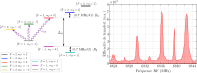
\includegraphics[width=\textwidth]{Fig/Modif_exp/levitation_RF.pdf}
\caption{\textbf{a: Principe de la spectroscopie radio-fréquences}. En balayant la fréquence de l'onde radio-fréquence appliquée, on adresse les différentes transitions entre sous-états Zeeman de $\protect\etatF{1}{}$ et $\protect\etatF{2}{}$ dont la séparation dépend du champ magnétique. \textbf{b: Spectre radio-fréquence.} Lorsque l'onde radio-fréquence est à résonance, on transfère des atomes initialement dans l'état $\protect\etatF{1}{}$ vers l'état $\protect\etatF{2}{}$. La présence de sept résonances équidistantes indique une dépolarisation du nuage, les règles de sélection imposant $\Delta \mf = \lbrace \pm 1,0 \rbrace$. Les trois premières résonances correspondent à celles illustrées sur la figure \textbf{a}. Le champ magnétique extrait de ce spectre est d'environ $\SI{4.4}{\gauss}$.}
\label{fig:calibration_RF}
\end{figure}



En relevant le spectre des transitions radio-fréquences\footnote{Cette mesure a été effectuée dans le piège dipolaire croisé, et étant donné le très grand désaccord du faisceau de piégeage, on peut considérer que les déplacements lumineux induits sur les états $\etatF{1}{}$ et $\etatF{2}{}$ sont identiques. La séparation entre les états considérés n'en sera donc pas affectée. Il est ensuite possible d'imager sélectivement les atomes transférés dans l'état $\etatF{2}{}$ par fluorescence en coupant la partie du faisceau d'imagerie provenant du laser repompeur.} en balayant la fréquence rayonnée $\nu_{\mathrm{RF}}$ comme illustré figure \ref{fig:calibration_RF}.b, on accède ainsi à la valeur du champ magnétique au niveau des atomes en déterminant $\delta\nu(B)$, qu'il est possible d'approximer par le décalage par effet Zeeman linéaire dans un régime de bas champ:
\begin{equation}
\delta \nu (B)\simeq -(m_{\mathrm{F_2}} - m_{\mathrm{F_1}} ) \times \SI{0.7}{\mega\hertz\per\gauss} \times B \text{ ,}
\label{eq:levitation_RF}
\end{equation}
où le champ $B$ correspond à la norme du champ magnétique total, c'est-à-dire le champ de biais étudié et les champs naturellement présents $\mathbf{b}_{\mathrm{0}}$: 
\begin{equation}
B=\sqrt{(b_{\mathrm{c,x}}+b_{\mathrm{0x}})^2+(B_{\mathrm{A}}+B_{\mathrm{B}}+b_{\mathrm{0y}})^2+(b_{\mathrm{c,z}}+b_{\mathrm{0z}})^2} \text{ .}
\end{equation}

En réalisant cette opération pour différents courants pour chacune des bobines de biais, il nous est possible de déterminer les calibrations des champs magnétiques \ref{eq:calibration_biais_lev} et \ref{eq:calibration_biais_comp}. En particulier, le comportement à très bas champ nous permet de déterminer les différentes composantes $b_{\mathrm{0i}}$ du champ rémanent, souvent négligeable devant le champ rayonné pour des courants usuels. L'ensemble des calibrations des champs de biais est alors donné table \ref{tb:levitation_RF}.
 

\renewcommand{\arraystretch}{1.1}
\begin{table}[!h]
{\rowcolors{2}{white}{MainColor!12}
\begin{center}
\begin{tabular}{ c|c }
%\hline
{\color{MainColor}\textbf{Grandeur}} & {\color{MainColor}\textbf{Valeur}} \\
%\hline
Calibration Biais A $c_{\mathrm{A}}$ & $\SI{4.70}{}\pm\SI{0.05}{\gauss\per\ampere}$ \\
%\hline
Calibration Biais B $c_{\mathrm{B}}$ & $\SI{6.18}{}\pm\SI{0.06}{\gauss\per\ampere}$ \\
%\hline
Calibration Compensation X $c_{\mathrm{x}}$ & $\SI{4.90}{}\pm\SI{0.05}{\gauss\per\ampere}$ \\
%\hline
Calibration Compensation Z $c_{\mathrm{z}}$ & $\SI{4.97}{}\pm\SI{0.05}{\gauss\per\ampere}$ \\
%\hline
Courant seuil Biais A $I_{\mathrm{0,A}}$ & $< \SI{1}{\milli\ampere}$ \\
%\hline
Courant seuil Biais B $I_{\mathrm{0,B}}$ & $\SI{0.345}{}\pm\SI{0.003}{\ampere}$ \\
%\hline
Champ rémanent $b_{\mathrm{0x}}$ & $\SI{0.089}{}\pm\SI{0.002}{\gauss}$ \\
%\hline
Champ rémanent $b_{\mathrm{0y}}$ & $\SI{0.426}{}\pm\SI{0.002}{\gauss}$ \\
%\hline
Champ rémanent $b_{\mathrm{0z}}$ & $\SI{-0.416}{}\pm\SI{0.002}{\gauss}$ \\
%\hline
\end{tabular}
\end{center}}
\caption{\textbf{Calibration des champs de biais dans la chambre de science.} Les champs rémanents $b_{\mathrm{0i}}$ correspondent aux champs extérieurs dans la direction $\vec{i}$. Le champ magnétique généré dans la cellule est proportionnel au courant parcourant les bobines $B_{\mathrm{i}} = c_{\mathrm{i}} \times (I_{\mathrm{i}}-I_{\mathrm{0,i}})$ avec $I_{\mathrm{0,i}}$ le courant seuil, qui correspond à la consigne minimale à appliquer pour que le courant circule dans les bobines.}
\label{tb:levitation_RF}
\end{table}
















\subsection{\'Etude du potentiel de lévitation}
\label{sc:oscillations_levitation}
Nous l'avons mentionné précédemment, il est important de maîtriser le potentiel de lévitation en fonction des différents champs magnétiques. Cette considération est d'autant plus importante dans la mesure où nous envisageons de réaliser un passage adiabatique d'une lévitation au champ magnétique magique, à bas champ, à une lévitation très décomprimée à fort champ. 

Dans cette section, nous allons donc caractériser le potentiel de lévitation en terme de fréquence de piégeage et de centre du potentiel. Nous pourrons ainsi calibrer le gradient magnétique généré par les bobines de gradient ainsi que les courbures des champs magnétiques générés par les bobines de biais. Nous soulignerons ensuite leur effet sur la position du centre du potentiel de lévitation et témoignerons ainsi de l'importance capitale des champs de compensation.




\paragraph*{Potentiel de lévitation}
Comme nous l'avons mentionné dans le chapitre précédent, il existe une limite pour les fréquences de piégeage (formule \ref{eq:theoreme_wing}) qui décroît avec la norme du champ magnétique. Une stratégie usuelle est donc de créer un champ aussi fort que possible, qui est d'environ \SI{2000}{\gauss} avec notre système (correspondant à un courant maximal de \SI{200}{\ampere}). Pour de tels champs, le potentiel magnétique n'est plus décrit par l'effet Zeeman linéaire, mais par la formule de Breit-Rabi \ref{eq:Breit-Rabi}. En revanche, pour une petite zone autour du centre du potentiel de lévitation, on peut simplifier l'étude en supposant que le champ change peu $B\simeq \Bzero$. On peut ainsi définir un facteur de Landé local:
\begin{equation}
\gftilde(\Bzero)=\frac{1}{\mf \mub} \frac{\mathrm{d}E}{\mathrm{d}B}(\Bzero) \text{ ,}
\label{eq:facteur_lande_local}
\end{equation}
obtenu à l'aide d'un développement limité de la formule de Breit-Rabi \ref{eq:Breit-Rabi} autour du champ $\Bzero$. La physique derrière cette approche est de considérer l'effet Zeeman linéaire sur un état dont la susceptibilité magnétique dépend du champ de Biais $\Bzero$. Cela se traduit par une correction du potentiel magnétique \ref{eq:potentiel_mag} qu'il est possible de réécrire sous la forme:
\begin{equation}
U_{\mathrm{mag}}(\mathbf{x})=m_{\mathrm{F}}\gftilde(\Bzero)\mub B(\mathbf{x}) \text{ ,}
\label{eq:potentiel_levitation}
\end{equation}
dans une zone proche autour du centre du potentiel de lévitation.


\begin{figure}
\centering
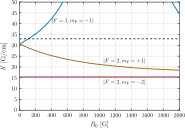
\includegraphics[width=0.7\textwidth]{Fig/Modif_exp/levitation_etats.pdf}
\caption{\textbf{Gradient nécessaire pour compenser la gravité en fonction du biais magnétique.} La valeur du gradient magnétique à appliquer pour léviter dépend de l'état électronique, mais aussi du biais magnétique $\protect\Bzero$ par la formule de Breit-Rabi. L'état $\protect\etatF{1}{-1}$ ne peut être lévité qu'à bas champ (courbe bleue), l'alimentation des bobines de gradient ne pouvant délivrer plus de \SI{50}{\ampere} (limite tracée en pointillés). Les états $\protect\etatF{2}{+1}$ (courbe marron) et $\protect\etatF{2}{-2}$ (courbe bordeaux) peuvent être lévités pour n'importe quelle valeur du biais. Les carrés correspondent aux différentes configurations expérimentales d'intérêt pour cette thèse.}
\label{fig:levitation_etats}
\end{figure}

\paragraph*{Gradient de lévitation}
À l'aide du potentiel \ref{eq:potentiel_levitation}, il nous est possible de déterminer la valeur du gradient magnétique nécessaire pour compenser la gravité:
\begin{equation}
b'=\frac{mg}{\mf \gftilde(\Bzero) \mub} \text{ ,}
\label{eq:gradient_levitation}
\end{equation}
qui, de manière générale, dépend donc du biais magnétique au niveau des atomes.
Cette dépendance est illustrée figure \ref{fig:levitation_etats} pour les différents états internes d'intérêt dans cette thèse: $\etatF{1}{-1}$, $\etatF{2}{+1}$ et $\etatF{2}{-2}$. 

Notons trois résultats remarquables de la figure \ref{fig:levitation_etats}: 
\begin{itemize}
\item[\textendash] L'état $\etatF{2}{-2}$ nécessite un gradient indépendant du biais magnétique pour être lévité. 
\item[\textendash] Les états $\etatF{1}{-1}$ et $\etatF{2}{+1}$ sont lévités pour le même gradient à bas champ. Plus précisément, la susceptibilité magnétique de ces états est égale uniquement pour un \emph{champ magnétique magique} $\magicB=\SI{3.229}{\gauss}$\footnote{Ce champ magique est dû au spin nucléaire. Une dérivation de ce champ peut être trouvée dans la référence \citep{denechaud2018vers}.}, impliquant que ces états \emph{d'horloge} ont le même comportement magnétique \citep{sarkany2014controlling}. Cela se traduit notamment par une lévitation simultanée de ces états.
\item[\textendash] L'état $\etatF{1}{-1}$ ne peut être lévité que pour des champs inférieurs à environ \SI{150}{\gauss} en raison de la limitation de courant (\SI{50}{\ampere}) de l'alimentation des bobines de gradient. En effet, le gradient nécessaire pour contrer la gravité augmente avec le champ magnétique.
\end{itemize}
Plusieurs stratégies expérimentales de lévitation s'offrent alors. La première provient de l'état $\etatF{2}{-2}$ qui peut être lévité à l'aide du bon gradient magnétique tout en gardant la valeur du champ de biais comme un degré de liberté. On peut alors fortement augmenter le champ de biais afin de réaliser des lévitations très décomprimées (carré bordeaux de la figure \ref{fig:levitation_etats}). Il s'agit de l'approche utilisée pour la mesure du temps de diffusion élastique, présentée chapitre \ref{ch:TauS_PRL}. Une autre possibilité est que les états d'horloge $\etatF{1}{-1}$ et $\etatF{2}{+1}$ peuvent coexister dans le champ de lévitation, on peut ainsi utiliser l'état interne de l'atome comme degré de liberté tout en étant lévité (carré bleu). Cette stratégie a par exemple été utilisée pour la mesure des fonctions spectrales \citep{volchkov2018measurement}.



Enfin, il est possible de déduire une calibration des bobines de gradient de la relation \ref{eq:gradient_levitation} entre le gradient magnétique et le biais $\Bzero$. En identifiant des couples $\lbrace I_{\mathrm{Gradient}}, I_{\mathrm{Biais}} \rbrace$ permettant de compenser précisément la gravité, on parcourt ainsi la courbe de la figure \ref{fig:levitation_etats} pour l'état $\etatF{1}{-1}$. On détermine alors le facteur de calibration $c_{\mathrm{G}}=0.66\pm\SI{0.01}{\gauss\per\centi\metre\per\ampere}$.




\paragraph*{Fréquences de la lévitation}
De manière générale, nous avons besoin de caractériser le piégeage résiduel de la lévitation, celui-ci pouvant influencer un piège optique fortement décomprimé dans une configuration à bas champ, et il est nécessaire d'estimer le potentiel résiduel des atomes en expansion dans le désordre dans le cas d'une configuration à fort champ.

Pour l'état $\etatF{1}{-1}$ en particulier, état d'horloge dans lequel nous créons notre condensat de Bose-Einstein\footnote{L'étude des oscillations est ici menée avec l'état $\etatF{1}{-1}$, mais peut être étendue aux autres états.}, le centre de masse du nuage décrit des oscillations autour du centre du potentiel de lévitation dont les fréquences peuvent être trouvées à l'aide de la norme du champ magnétique \ref{eq:norme_levitation} et du potentiel magnétique \ref{eq:potentiel_levitation}:
\begin{equation}
\omega_x^2=\omega_z^2=\left| \frac{\mf \gftilde \mub}{m} \left( \frac{b'^2}{4 \Bzero} - b'' \right) \right|
\quad \text{et} \quad
\omega_y^2= \left| \frac{2 \mf \gftilde \mub }{m} b'' \right| \text{ .}
\label{eq:frequences_leviation}
\end{equation}
Nous allons donc utiliser ces oscillations naturelles du nuage (une fois relâché après extinction du piège dipolaire) dans le piège de la lévitation magnétique pour caractériser le potentiel de lévitation en terme de centre et de courbure.%L'exploitation de ces oscillations fournit donc de précieux renseignements quant à la position du centre de la lévitation, mais aussi quant à la forme du potentiel magnétique dans lequel les atomes évoluent. 

En particulier, la mesure des fréquences du potentiel de lévitation permet de déterminer la courbure des champs générés par les bobines de biais A et de biais B. L'influence de ces courbures est représentée figure \ref{fig:frequences_levitation} pour les champs de biais A et de biais B. Pour un courant suffisamment grand, le terme de courbure $b_{\mathrm{i}}''= c_{\mathrm{i}}'' \times (I_{\mathrm{i}}-I_{\mathrm{0,i}})$ n'est plus négligeable devant celui de gradient, atténué par le biais. En effet, la comparaison des fréquences expérimentales aux fréquences \ref{eq:frequences_leviation} à courbure nulle $b''=0$ montre un désaccord significatif dans la zone des courants les plus hauts, tandis qu'un modèle tenant compte d'une courbure proportionnelle au courant décrit correctement cette zone (voir figure \ref{fig:frequences_levitation}.b). On peut alors extraire le facteur de conversion courbure/courant $c_{\mathrm{i}}''$, dont les valeurs sont données dans la table \ref{tb:courbures_levitation}.




\begin{figure}
\centering
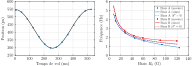
\includegraphics[width=\textwidth]{Fig/Modif_exp/oscillation_levitation.pdf}
\caption{\textbf{a: Oscillation du nuage dans la lévitation magnétique.} Le nuage, initialement dans le piège optique, est relâché décentré par rapport au potentiel de la lévitation. Il acquiert alors un mouvement oscillatoire autour du centre de la lévitation pendant le temps où la gravité est compensée. \textbf{b: \'Evolution des fréquences de piégeage de la lévitation.} Les fréquences mesurées (points) diminuent avec l'augmentation de $\Bzero$ et sont comparées à des simulations du potentiel (lignes continues) afin de calibrer le champ créé par les bobines. L'influence des courbures est visible pour les plus champs les plus intenses, les simulations en absence de courbure (courbes tiretées) montrant alors une déviation par rapport aux données.}
\label{fig:frequences_levitation}
\end{figure}


%\renewcommand{\arraystretch}{1.1}
\begin{table}[!h]
\begin{center}
{\rowcolors{2}{white}{MainColor!12}
\begin{tabular}{ c|c }
%\hline
{\color{MainColor} \textbf{Courbure}} & {\color{MainColor} \textbf{Valeur}} \\
%\hline
Gradient $c_{\mathrm{G}}$ & $0.66\pm\SI{0.01}{\gauss\per\centi\metre\per\ampere}$ \\
%\hline
Biais A $c_{\mathrm{A}}''$ & $\SI{4e-2}{}\pm\SI{1e-2}{\gauss\centi\metre^{-2}\ampere^{-1}}$ \\
%\hline
Biais B $c_{\mathrm{B}}''$ & $\SI{-7e-2}{}\pm\SI{1e-2}{\gauss\centi\metre^{-2}\ampere^{-1}}$ \\
%\hline
\end{tabular}}
\end{center}
\caption{\textbf{Calibration du potentiel de lévitation magnétique.} Les bobines de gradient créent un champ quadrupolaire, dont le gradient vertical permet de faire léviter les atomes. Celui-ci est relié au courant parcourant les bobines selon $b'=c_{\mathrm{G}}\times I_{\mathrm{G}}$. Les bobines de lévitation générant les champs de biais n'étant pas en configuration de Helmholtz, elles créent donc une courbure de champ magnétique au niveau des atomes. Cette courbure dépend de la géométrie des bobines ainsi que du courant les parcourant $b_{\mathrm{i}}''= c_{\mathrm{i}}'' \times (I_{\mathrm{i}}-I_{\mathrm{0,i}})$.}
\label{tb:courbures_levitation}
\end{table}

On peut alors estimer les fréquences du potentiel de lévitation dans les configurations expérimentales d'intérêt, identifiées par des carrés sur la figure \ref{fig:levitation_etats}. Pour la configuration à bas champ (carré bleu), c'est-à-dire au champ magique $\magicB$, les états $\etatF{1}{-1}$ et $\etatF{2}{+1}$ sont soumis à un piégeage de fréquence d'environ \SI{5}{\hertz} par les bobines de biais A. Dans le régime de champ fort, nécessaire pour obtenir les décompressions maximales qu'offre notre système, la fréquence de piégeage de l'état $\etatF{2}{+1}$ est diminuée jusqu'à \SI{0.20}{\hertz} sous un champ de \SI{2000}{G} (carré marron), tandis que la fréquence d'anti-piégeage de l'état $\etatF{2}{-2}$ atteint \SI{0.18}{\hertz} (carré bordeaux) \citep{bernard2010transport}.





\paragraph*{Centre de la lévitation}
Dans le cas d'un système idéal, le centre du potentiel magnétique correspond au centre géométrique des bobines. Cependant, on comprend aisément qu'en raison du gradient magnétique de lévitation, la position horizontale du centre du potentiel magnétique sera très sensible aux perturbations extérieures ainsi qu'aux défauts de positionnement des bobines\footnote{Le champ de biais généré par les bobines de lévitation n'est pas orienté parfaitement selon l'axe du gradient vertical. L'effet d'un angle $\theta$ avec la direction verticale se manifeste via la présence d'un champ horizontal $\Bzero \sin{\theta}$, qui participe à déplacer le centre du potentiel.}. En particulier, on peut s'attendre à ce qu'un champ horizontal $b_{\mathrm{z}}$ entraîne un déplacement $\Delta z=-2b_{\mathrm{z}}/b'$ du centre du potentiel. Afin d'éviter de mettre le nuage en mouvement après relâchement du piège optique, on utilise alors des champs de compensation générés à l'aide de bobines supplémentaires, représentées en violet et en noir figure \ref{fig:geometrie_levitation}, dont le rôle est de repositionner le centre du potentiel magnétique sur le nuage. 

Le champ permettant de déplacer le potentiel est donc la somme d'un champ naturellement présent et du champ de compensation:
\begin{equation}
b_{\mathrm{i}}=b_{\mathrm{0,i}}+c_{\mathrm{c,i}} \times I_{\mathrm{c,i}} \quad \text{avec} \quad i=\lbrace x,z \rbrace \text{ .}
\end{equation}
Les mesures des différents termes de ce champ ont été effectuées à l'aide de radio-fréquences, comme décrit section \ref{sc:levitation_RF}. 

Il est alors possible de généraliser l'expression \ref{eq:champ_mag_levitation} du champ magnétique total sous l'effet d'une petite composante suivant l'axe horizontal $\vec{z}$\footnote{Nous illustrons ici l'effet d'un champ horizontal dirigé uniquement suivant la direction $\vec{z}$, la démarche étant identique dans le cas d'un champ orienté suivant la direction $\vec{x}$.}:
\begin{equation}
\mathbf{B}=\left( \frac{b'}{2}x \right) \vec{x} + \left[ \Bzero - b'y + b'' \left( y^2 - \frac{x^2+z^2}{2} \right) \right] \vec{y} + \left( \frac{b'}{2}z +b_{\mathrm{z}} \right) \vec{z} \text{ .}
\end{equation}
En calculant la norme de ce champ, on détermine alors que la présence d'un champ de biais $b_{\mathrm{z}}$ dans le plan horizontal mène à un déplacement du centre du potentiel
\begin{equation}
\Delta z =-\frac{2b_{\mathrm{z}}}{b'}\left( \frac{1}{1-4\Bzero b'' /b'^2} \right)
\end{equation}
pour un champ $b_{\mathrm{z}} \ll \Bzero$. Dans le régime de bas champ $\Bzero$, on retrouve ainsi le résultat intuitif annoncé précédemment: l'effet d'un biais horizontal est de déplacer le centre de la lévitation à l'aide d'un gradient $b'/2$, résultant en un déplacement du potentiel magnétique de $\Delta z =-2b_{\mathrm{z}}/b'$. 

Une conséquence importante de ce résultat est que le déplacement du centre de la lévitation par un biais de positionnement dépend du biais de lévitation, ainsi que du gradient et de la courbure du champ. La décompression adiabatique de la lévitation magnétique peut alors entraîner un déplacement du centre du potentiel de lévitation. La connaissance du déplacement du centre du potentiel en fonction des différents paramètres nous permettra alors de contrôler la position de ce dernier à l'aide des champs de compensation.

L'étude du système de lévitation magnétique nous a non seulement permis de calibrer les champs magnétiques générés par nos bobines dont la position, l'orientation et le comportement magnétique ont été légèrement modifiés suite à un démontage et de lourds travaux de réparation, mais elle nous a de plus permis de caractériser le potentiel de lévitation, dont la connaissance fine est cruciale à bas champ comme à fort champ. Les conclusions de cette étude nous ont mené à faire l'acquisition d'alimentations \emph{Toellner TOE 8851-40} pour les champs de compensation. En effet, il nous sera nécessaire de pouvoir contrôler de manière arbitraire les courants des bobines de compensation en cours de séquence, ce que les alimentations précédentes ne permettaient pas.





















\section{Changement du laser infrarouge et calibration du piège optique}
%Listés dans la partie \ref{sc:chambre_science}, u
Uniquement deux éléments participent à la manipulation d'atomes dans la chambre de science avant condensation. Le premier élément, la lévitation magnétique, a fait l'objet de l'étude présentée dans la partie précédente. 

Cette partie se concentrera sur le second élément, le piège optique. Nous commencerons par présenter le système optique et décrire les changements opérés, puis nous décrirons la calibration de ce piège sur les atomes.

\subsection{Changement du laser infrarouge fibré Ytterbium }
Dans le chapitre précédent, nous avons vu que le piège dipolaire était composé de deux faisceaux se croisant dans la chambre de science. Ces deux faisceaux, la pince et le dimple, sont orientés suivant les directions $\vec{z}$ et $\vec{y}$ respectivement et permettent de franchir le seuil de condensation. Il s'agit donc du piège donnant au condensat ses propriétés. De plus, c'est avec ce même piège que l'on met en œuvre les techniques de refroidissement extrêmes que sont l'ouverture adiabatique du piège ou encore le refroidissement par delta-kick. Il est donc primordial d'avoir une connaissance complète des caractéristiques de ce piège.



Les deux faisceaux du piège dipolaire croisé proviennent d'une source laser commune avant d'être mis en forme séparément. Cette source, un laser fibré Ytterbium de \emph{Keopsys} émettant une puissance initiale de \SI{20}{\watt} en continu à une longueur d'onde $\lambda=\SI{1070}{\nano\metre}$, a été remplacée au cours de ma thèse. Ce laser a été sujet à un grand nombre d'opérations de maintenance, et, dans les mois précédant son changement, il ne pouvait plus émettre que \SI{14}{\watt} lors de son allumage et seulement \SI{12.5}{\watt} en fin de journée.
 
Cette source a été remplacée par un laser fibré Ytterbium \emph{YLR-50-LP-A-Y12} de \emph{IPG}, opérant à la même longueur d'onde $\lambda=\SI{1070}{\nano\metre}$, et avec une puissance maximale mesurée à \SI{55}{\watt}. La taille du faisceau en sortie de fibre est de \SI{0.8}{\milli\metre} (contre \SI{1.4}{\milli\metre} pour le laser Keopsys), il a donc fallu adapter un télescope afin de conserver les mêmes tailles de faisceaux au niveau des atomes. Le montage de mise en forme des faisceaux est présenté figure \ref{fig:optique_1070}. Celui-ci est majoritairement mis dans des tubes\footnote{Seule la zone du montage dédiée à l'asservissement de puissance n'est pas mise sous tube. La zone sous tube s'arrête au niveau du modulateur acousto-optique, puis reprend au niveau du second télescope, voir figure \ref{fig:optique_1070}.} contenant un grand nombre de diaphragmes, facilitant ainsi la procédure d'alignement.

\begin{figure}
\centering
\includegraphics[width=0.95\textwidth]{Fig/Modif_exp/optique_1070_new_style.pdf}
\caption{\textbf{Schéma du montage optique pour le piège dipolaire.} Le faisceau issu du laser source passe dans un premier télescope avant d'être séparé en deux parties. La partie déviée passe dans une fibre optique pour devenir le faisceau de la pince. La partie transmise passe ensuite dans un second télescope pour devenir elliptique et arrive dans la \emph{Dimple box}, qui transmet le faisceau jusqu'aux atomes et contient les optiques d'imagerie \citep{muller2015coherent}. Afin de garder les mêmes tailles de faisceaux, la première lentille du premier télescope, de focale +\SI{175}{\milli\metre}, a été remplacée par une lentille de focale +\SI{100}{\milli\metre}.}
\label{fig:optique_1070}
\end{figure}

\begin{figure}
\centering
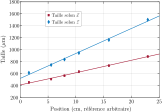
\includegraphics[width=0.7\textwidth]{Fig/Modif_exp/expansion_dimple.pdf}
\caption{\textbf{Évolution des tailles du faisceau dimple après la cellule.} Les tailles du faisceau dimple sont représentées en fonction de la position de la caméra (points). La divergence du faisceau permet de remonter aux waists du faisceau et d'en estimer la position. Les waists extraits par ajustement (lignes continues) sont de $\mathrm{w_z}\simeq \SI{82}{\micro\metre}$ et de $\mathrm{w_x}\simeq \SI{160}{\micro\metre}$ et leur position est compatible avec celle des atomes.}
\label{fig:taille_dimple}
\end{figure}

\paragraph*{Estimation de la taille du faisceau dimple au niveau des atomes}
L'utilisation d'une fibre optique pour la mise en forme du faisceau de la pince permet de s'assurer que le mode envoyé sur les atomes n'a pas changé. Pour le faisceau dimple en revanche, le trajet jusqu'à la cellule se fait en espace libre. Celui-ci est rendu elliptique à l'aide d'un second télescope, comportant quatre lentilles dont deux cylindriques, comme illustré figure \ref{fig:optique_1070}. Le rapport d'aspect du faisceau est alors de 2. 




L'estimation de la taille du faisceau au niveau des atomes est réalisée en étudiant l'évolution de son profil d'intensité lumineuse après le passage au travers de la cellule. 
Cette estimation est aisée pour des faisceaux gaussiens: la taille du faisceau $\mathrm{w}_{\mathrm{i}}(y)$ dans la direction $\vec{i}$ ($\vec{i}= \lbrace \vec{x},\vec{z} \rbrace$) est donnée par:
\begin{equation}
\mathrm{w}_{\mathrm{i}}(y)=\mathrm{w}_{\mathrm{i}} \sqrt{1+\left( \frac{y-y_0}{y_{\mathrm{Ri}}} \right)^2} \text{ ,}
\label{eq:taille_faisceau}
\end{equation}
où $y_0$ correspond à la position pour laquelle la taille du faisceau $\mathrm{w}_{\mathrm{i}}(y_0)=\mathrm{w}_{\mathrm{i}}$ est minimale et $\mathrm{w}_{\mathrm{i}}$ est le waist du faisceau. La distance de Rayleigh associée s'exprime $y_{\mathrm{Ri}}=\pi \mathrm{w}_{\mathrm{i}}^2 / \lambda$ et correspond à la distance sur laquelle la taille du faisceau suivant la direction $\vec{i}$ change peu. Dans le régime de champ lointain $y-y_0 \gg y_{\mathrm{Ri}}$, le faisceau diverge selon un angle $\tan \theta_{\mathrm{i}} \simeq \lambda / \pi \mathrm{w}_{\mathrm{i}}$.

La mesure des tailles du faisceau a été réalisée à l'aide d'une caméra \emph{IDS Ueye} disposant d'une matrice de $1024 \times 1280$ pixels de \SI{5.2}{\micro\metre} de côté. Les tailles ont été extraites par ajustement gaussien d'un profil unidimensionnel d'intensité lumineuse obtenu par intégration suivant une direction. Enfin, l'évolution de la taille en fonction de la position a été ajustée par la formule \ref{eq:taille_faisceau}, illustrée figure \ref{fig:taille_dimple}.



On estime alors les waists du faisceau dimple à $\mathrm{w_z}=81.6\pm\SI{7.8}{\micro\metre}$ et $\mathrm{w_x}=160\pm \SI{13}{\micro\metre}$, proches des valeurs de la configuration précédant le changement du laser source. La position $y_0$ de ces waists est compatible avec la position des atomes, et la longueur de Rayleigh du faisceau est de l'ordre de $y_{\mathrm{Rz}}\simeq \SI{2}{\centi\metre}$.



\subsection{Calibration du piège optique}
\label{sc:calibration_piege_optique}
%L'utilisation d'une fibre optique pour la mise en forme du faisceau de la pince permet de s'assurer que le mode envoyé sur les atomes n'a pas changé. Pour le faisceau dimple en revanche, le trajet jusqu'à la cellule se fait sans filtrage. La présence de deux périscopes, d'un nombre d'éléments optiques important et l'utilisation d'un profil elliptique imposent une étude attentive des caractéristiques de ce faisceau au niveau des atomes.

La caractérisation finale du piège dipolaire croisé se fait à l'aide des fréquences de piégeage, qui fixent les propriétés physiques du nuage. %Afin de mesurer ces fréquences, nous avons fait le choix d'induire de petites oscillations du nuage à l'intérieur du piège à l'aide d'une force extérieure, et de suivre ces oscillations en fonction du temps d'évolution dans le piège de manière équivalente à celle présentée pour la lévitation magnétique section \ref{sc:oscillations_levitation}. 


\paragraph*{Calibration des fréquences de piégeage}
Le fonctionnement du piège optique repose sur le potentiel dipolaire. Celui-ci s'écrit:
\begin{equation}
U(\mathbf{r})=\frac{3 \pi c^2 \Gamma}{2 \omega_0^3 \overline{\Delta}} I(\mathbf{r}) \quad \text{avec} \quad \frac{1}{\overline{\Delta}}=\frac{1}{\omega-\omega_0}-\frac{1}{\omega+\omega_0} \text{ .}
\end{equation}
Les faisceaux utilisés étant de forme gaussienne, on peut ainsi exprimer la profondeur de piégeage de chaque faisceau:
\begin{equation}
U_{\mathrm{pince}}= \frac{3c^2 \Gamma }{\omega_0^3 \overline{\Delta}} \frac{P_{\mathrm{pince}}}{\mathrm{w}_0^2} \quad \text{et} \quad U_{\mathrm{dimple}}=\frac{3c^2 \Gamma }{\omega_0^3 \overline{\Delta}}\frac{P_{\mathrm{dimple}}}{\mathrm{w}_{\mathrm{x}} \mathrm{w}_{\mathrm{z}}} \text{ .}
\label{eq:profondeur_piege_optique}
\end{equation}
En supposant que les atomes restent proches du centre du piège, on peut de plus faire l'approximation que le profil d'intensité des faisceaux est de forme harmonique. On définit ainsi les fréquences de piégeage $\omega_{x,y,z}$ par analogie avec un oscillateur harmonique. Rappelons que le confinement dans les directions $\vec{x}$ et $\vec{y}$ est fait par la pince, et que celui dans la direction $\vec{z}$ est fait par le dimple, les fréquences de piégeage du piège dipolaire croisé s'expriment alors:
\begin{equation}
\omega_x=\omega_y=\sqrt{-\frac{4 U_{\mathrm{pince}}}{m \mathrm{w}_0^2}} \quad \text{et} \quad \omega_z=\sqrt{-\frac{4U_{\mathrm{dimple}}}{m \mathrm{w}_{\mathrm{z}}^2}} \text{ .}
\label{eq:frequences_piege_optique}
\end{equation}
%La caractérisation finale du piège dipolaire croisé se fait à l'aide des fréquences de piégeage, qui fixent les propriétés physiques du nuage. 
Afin de mesurer ces fréquences, nous avons fait le choix\footnote{Nous avons retenu la méthode de mesure des fréquences de piégeage à l'aide d'excitations dipolaires. Il est aussi possible de mesurer ces fréquences par excitations paramétriques à l'aide de petites modulations de la profondeur du piège \citep{savard1997laser}.} d'induire de petites oscillations du centre de masse du nuage à l'intérieur du piège à l'aide d'une force extérieure, et de suivre ces oscillations en fonction du temps d'évolution dans le piège de manière équivalente à celle présentée pour la lévitation magnétique section \ref{sc:oscillations_levitation}. En relevant la position des atomes en fonction de la durée d'évolution dans le piège après excitation, on extrait alors la fréquence associée à l'aide d'un ajustement illustré figure \ref{fig:frequences_piege_optique}.a.

\begin{figure}
\centering
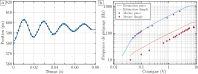
\includegraphics[width=\textwidth]{Fig/Modif_exp/frequences_piege_optique.pdf}
\caption{\textbf{a: Exemple d'oscillation dans le piège optique.} Le nuage oscille dans la direction $\vec{z}$ pour une puissance du faisceau dimple de \SI{0.70}{\watt} après avoir été poussé par un gradient magnétique (points bleus). La fréquence d'oscillation est alors de $\omega_z /2\pi \simeq \SI{51}{\hertz}$, extraite par ajustement (courbe noire). \textbf{b: Fréquences d'oscillations du piège optique.} Les fréquences mesurées par oscillations du nuage (points) sont tracées en fonction de la puissance du faisceau associé. Les valeurs des calibrations $A_{\mathrm{pince}}$ et $A_{\mathrm{dimple}}$ sont ensuite extraites par ajustement de ces données (lignes continues).}
\label{fig:frequences_piege_optique}
\end{figure}

La fréquence de piégeage dans les directions $\vec{x}$ et $\vec{y}$, liée à la pince optique, a pu être mesurée à l'aide de la lévitation magnétique. En commutant rapidement le courant des bobines de gradient, on dispose d'un bouton pour allumer et éteindre la gravité, et donc générer une force pendant un bref instant pour donner un mouvement aux atomes dans le piège. La mesure de la fréquence de piégeage dans la direction $\vec{z}$ a été effectuée selon deux méthodes en fonction de la puissance du faisceau dimple:
\begin{itemize}
\item[\textendash] À haute puissance, les atomes sont poussés à l'aide d'un gradient magnétique suivant la direction $\vec{z}$ provenant de bobines de compensation branchées en configuration anti-Helmholtz. Celles-ci peuvent exercer une force sur les atomes pendant de courts instants à l'aide d'un commutateur rapide.
\item[\textendash] À plus basse puissance, le piège optique est très décomprimé et peu profond. Cependant, le piégeage de la lévitation peut arracher les atomes du piège optique, il est donc nécessaire de déplacer le centre de la lévitation magnétique à l'aide de champs de compensation suivant la direction $\vec{z}$. Pour pousser les atomes, on utilise alors les bobines de compensation dans leur configuration normale, et leur brève extinction conduit à accélérer les atomes en déplaçant le centre de la lévitation magnétique.
\end{itemize}



L'évolution des fréquences de piégeage de chaque faisceau en fonction de la puissance optique est représentée figure \ref{fig:frequences_piege_optique}.b en échelle logarithmique. La variation des fréquences s'est faite en abaissant la puissance du laser au cours de l'évaporation optique, celle-ci conduisant à une décompression du piège de comportement $\omega /2\pi =A \sqrt{P}$ comme le témoignent les formules \ref{eq:profondeur_piege_optique} et \ref{eq:frequences_piege_optique}. Les fréquences mesurées expérimentalement (carrés pour la pince optique, losanges pour le faisceau dimple) sont ajustées par une loi de puissance (lignes continues). La calibration de la pince est alors déterminée à $A_{\mathrm{pince}}=980\pm \SI{20}{\hertz\per\watt^{1/2}}$, et celle du dimple à $A_{\mathrm{dimple}}=60.5\pm \SI{1.0}{\hertz\per\watt^{1/2}}$, proche de la valeur précédant le remplacement du laser source\footnote{La dernière calibration date de la mise en place de la \emph{dimple box} lors de la thèse de Kilian Muller \citep{muller2015coherent}. Celle du dimple était alors de $A_{\mathrm{dimple}}=64.5\pm \SI{1.2}{\hertz\per\watt^{1/2}}$.}.







%Une seconde conséquence de la figure \ref{fig:frequences_piege_optique} est que les deux faisceaux présentent une saturation à haute puissance, c'est à dire qu'ils restent à leur puissance maximale au delà d'une certaine consigne seuil. Pour le dimple, cette saturation provient d'une limitation de la puissance de la source de la radio-fréquence servant à la diffraction du faisceau dans le modulateur acousto-optique. Pour la pince, cette limitation provient du maximum de l'efficacité de diffraction du modulateur acousto-optique. Ces deux saturations peuvent être repoussées en augmentant la puissance émise par le laser source\footnote{Le réglage actuellement utilisé sur l'expérience est une émission à 50\% de la puissance maximale du laser \emph{IPG}, c'est à dire environ \SI{23}{\watt}. Il a été observé que le mode émis est suffisamment stable à ce point de fonctionnement.}, cependant elles ne sont pas problématiques pour notre configuration. De plus, cette augmentation de puissance se traduirait par un chauffage local des bloqueurs de faisceau plus important, entraînant des effets thermiques néfastes.












\section{Optimisation de l'évaporation tout-optique}
\label{sc:evap_optique}
Vingt-cinq ans après l'obtention du premier condensat de Bose-Einstein, l'étape de refroidissement par évaporation forcée reste un passage obligatoire pour l'obtention d'un gaz dégénéré, à l'exception de quelques développements récents se basant sur des techniques novatrices de refroidissement laser \citep{hu2017creation,stellmer2013laser}. 

Comme brièvement présenté dans le chapitre précédent, le principe du refroidissement évaporatif repose sur l'extraction de particules très énergétiques, suivie par la thermalisation des particules restantes moins énergétiques en moyenne, se traduisant donc par une diminution de la température. Néanmoins, l'efficacité de ce processus dépend fortement de la configuration expérimentale. Les modifications apportées à notre piège optique nécessitent donc d'adapter les consignes d'évaporation à notre nouvelle géométrie. %De plus, l'utilisation de nouvelles cartes analogiques \emph{National Instruments} avec la suite \emph{Cicero Word Generator} permet de générer de nouvelles consignes arbitraires, non limitées à des morceaux de rampes telles qu'auparavant. 

Dans cette partie, nous commencerons par présenter le fonctionnement du refroidissement par évaporation forcée, puis nous détaillerons les résultats de l'optimisation de notre évaporation optique dans un second temps.


\subsection{Lois d'échelle du refroidissement évaporatif}
\label{sc:scaling_laws_ohara}
Le but de l'étape de refroidissement évaporatif étant d'augmenter la densité dans l'espace des phases $\mathcal{D}=n \ldb^3$, aussi appelée \emph{paramètre de dégénérescence}, il est donc nécessaire que notre système présente de la dissipation afin de franchir le seuil de condensation \citep{metcalf2007laser}. L'origine de cette dissipation repose sur la profondeur finie des pièges utilisés.  

\paragraph*{Évaporation naturelle dans un piège de profondeur finie}
Une conséquence de cette profondeur finie est que la fonction de partition $f(E)$ est tronquée à l'énergie $U$ correspondant à la profondeur du piège. Plus précisément, il a été montré que la fonction de partition est très proche d'une distribution de Boltzmann tronquée \citep{luiten1996kinetic}:
\begin{equation}
f(E)\propto e^{-\frac{E}{\kB T}} \Theta(U-E) \text{ .}
\label{eq:fonction_partition}
\end{equation}
Le temps de convergence vers cette distribution, c'est-à-dire le temps de thermalisation $\tau_{\mathrm{th}}$, est de l'ordre de quelques collisions entres les particules du gaz, dont le taux s'exprime $\Gamma_{\mathrm{c}}=n \sigma \overline{v}$, avec $n$ la densité du gaz, $\sigma$ la section efficace de diffusion et $\overline{v}$ la vitesse moyenne relative entre deux atomes \citep{walraven2010elements}.

En effet, la collision de deux particules permet de transférer de l'énergie d'une particule à la seconde. En particulier, une particule est susceptible d'acquérir par collision une énergie mécanique totale supérieure à la profondeur de piège, celle-ci est donc extraite du piège et emporte une énergie $U+\kappa\kB T$ ($\kappa>0$) supérieure à l'énergie moyenne par particule. %La particule restante a quant à elle perdu de l'énergie. 

Ce processus étant le plus probable pour des particules de grandes énergies, celui-ci favorise l'accumulation des particules dans les états de basse énergie tandis qu'il dépeuple les états de grande énergie. Ce raisonnement permet d'expliquer de manière qualitative la forme de la fonction de partition \ref{eq:fonction_partition}, qui favorise les états de basse énergie.

Ce phénomène d'\emph{évaporation naturelle} conduit donc à une diminution de la température, dont l'efficacité décroît avec le refroidissement du nuage. En effet, l'énergie moyenne par particule diminuant, la probabilité que des particules acquièrent suffisamment d'énergie pour s'échapper du piège décroît exponentiellement \citep{walraven2010elements}. Ainsi, le processus d'évaporation naturelle est fortement ralenti et le taux d'évaporation, c'est-à-dire le nombre de particules expulsées du piège par évaporation naturelle par unité de temps, peut être estimé par 
\begin{equation}
\Gamma_{\mathrm{ev}}\sim e^{-U/\kB T} \Gamma_{\mathrm{c}} \text{ ,}
\label{eq:taux_evap}
\end{equation}
avec $\Gamma_{\mathrm{c}}$ le taux de collisions. Le taux d'évaporation devient ainsi exponentiellement petit, l'évaporation est alors figée. 	

%Très rapidement, le temps d'évaporation $1/\Gamma_{\mathrm{ev}}$ excède le temps de vie des atomes dans le piège et ceux-ci sont perdus par des collisions inélastiques. 
Afin de dépasser cette limitation et de garder une évaporation efficace, la technique expérimentale développée afin d'obtenir les premiers condensats de Bose-Einstein consiste à abaisser progressivement la profondeur du piège $U$. On parle alors d'\emph{évaporation forcée}.





\paragraph*{Lois d'échelle de l'évaporation forcée}
Comme mentionné précédemment, la mise en œuvre pratique du refroidissement évaporatif se fait par le biais de la diminution de la profondeur du piège, forçant ainsi le processus d'évaporation. Cette opération est réalisée en continu, et à une vitesse suffisamment lente devant le temps de thermalisation $\tau_{\mathrm{th}}$ afin que le système soit constamment à l'équilibre thermodynamique\footnote{Dans ce cas, les seules pertes d'atomes considérées sont celles liées à l'évaporation par collisions. Cela revient à négliger la dynamique de thermalisation de l'évaporation, qui fait apparaître les pertes par déversement\citep{cohen1996atomes}. Celles-ci correspondent aux atomes ayant une énergie de $U-\delta E$ qui ne sont plus piégés lors de l'abaissement de la profondeur du piège de $U$ à $U-\mathrm{d}U$, avec $\mathrm{d}U > \delta E$. Dans le cas d'un gaz à l'équilibre thermodynamique, seule une infime partie des atomes se trouve dans cet intervalle d'énergie que l'on peut négliger devant les autres sources de pertes.}. 


On pressent à l'aide de l'équation \ref{eq:taux_evap} que le rapport entre la profondeur du piège et la température du gaz piégé joue un rôle fondamental dans l'évaporation. On définit alors le paramètre de troncature $\eta$:
\begin{equation}
\eta=\frac{U}{\kB T} \text{ .}
\end{equation}
Dans le cas d'un abaissement lent et continu de la profondeur du piège, le paramètre de troncature est approximativement constant\footnote{Étant donné la dépendance exponentielle du taux d'évaporation en $\eta$, le processus d'évaporation sera très fortement ralenti dans le cas d'un nuage très froid ($\eta$ grand), et rapide dans le cas d'un nuage chaud ($\eta$ petit). Lors de l'abaissement progressif de la profondeur du piège, la température va donc varier avec la profondeur du piège.} et sa valeur est de l'ordre de $\eta\approx 10$ dans le cas d'un piège optique.



Le potentiel de piégeage $U(\mathbf{x},t)$ étant modifié au cours de l'évaporation, les atomes sont soumis à un potentiel variant dans le temps. Dans le cas d'un piège harmonique, les fréquences de piégeage associées peuvent changer au cours de l'évaporation en fonction de l'implémentation expérimentale du refroidissement évaporatif. %\footnote{La méthode de couteau radio-fréquence utilisée dans le piège magnétique dans la première chambre ne modifie pas les fréquences de piégeages et ne change que la profondeur du piège, tandis que l'évaporation tout optique, réalisée à l'aide de faisceaux lasers de tailles fixées, est accompagnée d'une décompression du piège lors de l'abaissement de la puissance des lasers.}
Les variations de la géométrie du piège sont alors caractérisées par le paramètre $\nu$ défini par
\begin{equation}
\nu=\frac{\dot{\overline{\omega}}/\overline{\omega}}{\dot{U}/U}
\end{equation}
où $\overline{\omega}$ est la moyenne géométrique des fréquences du piège. Comme explicité formule \ref{eq:frequences_piege_optique}, les fréquences de piégeage du piège optique évoluent en $\overline{\omega}\propto\sqrt{U}$, impliquant donc $\nu=0.5$ \citep{o2001scaling}. L'abaissement de la profondeur du piège sera donc forcément accompagnée d'une décompression de celui-ci. 




Dressons alors un bilan d'énergie afin de déterminer la manière dont varient les principales quantités thermodynamiques au cours de l'évaporation. L'énergie totale du gaz dans un piège harmonique est donnée par
\begin{equation}
E=3N\kB T
\end{equation}
avec $N$ le nombre total d'atomes. La variation temporelle de l'énergie totale du gaz est alors donnée par
\begin{equation}
\dot{E}=3\dot{N} \kB T + 3 N \kB \dot{T} \text{ ,}
\label{eq:variation_energie_derivee}
\end{equation}
exprimée en fonction des variations temporelles du nombre d'atomes et de la température.

En identifiant les différentes sources de variations de l'énergie totale, on montre que la variation de l'énergie totale du système est donnée par \citep{cohen1996atomes}
\begin{equation}
\dot{E}=\dot{N}(U+\kappa \kB T) +\nu\frac{\dot{U}}{U}E \text{ ,}
\label{eq:variation_energie_bilan}
\end{equation}
où le premier terme décrit la perte d'énergie liée à l'évaporation des atomes énergétiques et le second terme représente le changement d'énergie potentielle des particules restées dans le piège, traduisant la décompression de ce dernier. Dans le cas d'une évaporation 3D, $\kappa=3/2$ \citep{ketterle1996evaporative}.

En combinant les équations \ref{eq:variation_energie_derivee} et \ref{eq:variation_energie_bilan}, on montre alors que la variation du nombre d'atomes en fonction de la profondeur de piégeage est donnée par \citep{o2001scaling}:
\begin{equation}
\frac{\dot{N}}{N}={\frac{3(1-\nu)}{\eta'-3}} \frac{\dot{U}}{U} \text{ ,}
\label{eq:nombre_atome_evap}
\end{equation}
avec $\eta'=\eta+\kappa$. Il est alors possible de déterminer les lois d'échelle des différentes grandeurs thermodynamiques d'un gaz classique. 

En particulier, dans le cas d'un piège harmonique, la densité dans l'espace des phases s'exprime:
\begin{equation}
\mathcal{D}=N\left(\frac{\hb \overline{\omega}}{\kB T}\right)^3 \text{ .}
\end{equation}
On peut alors déterminer les variations du paramètre de dégénérescence en fonction des variations du nombre d'atomes: 
\begin{equation}
\frac{\dot{\mathcal{D}}}{\mathcal{D}} = -\gamma \frac{\dot{N}}{N} \text{ .}
\label{eq:efficacite_evaporation}
\end{equation}
Le paramètre $\gamma=\eta'-4$ correspond à l'efficacité du processus d'évaporation: la perte d'atomes engendre un gain de densité dans l'espace des phases d'autant plus élevé que ce paramètre est grand. L'enjeu de l'optimisation du refroidissement évaporatif consiste donc à augmenter cette efficacité autant que possible.

Une conséquence remarquable de l'équation \ref{eq:efficacite_evaporation} est que l'efficacité du processus d'évaporation ne dépend pas du paramètre $\nu$ témoignant du changement de forme du piège. Ceci s'explique par le fait que pour une évaporation à $\eta$ constant, le paramètre $\nu$ traduit une ouverture adiabatique du piège, la décompression du nuage étant accompagnée d'une diminution de la température, voir section \ref{sc:chambre_science}. 


\paragraph*{Taux de collisions et régime d'emballement}
Si l'équation \ref{eq:efficacite_evaporation} ne fait pas apparaître l'influence du paramètre $\nu$, celui-ci joue cependant un rôle primordial quant à la cinétique de l'évaporation. En effet, la vitesse maximale d'évaporation est limitée par la vitesse à laquelle le gaz atteint un état d'équilibre thermique, c'est-à-dire le taux de thermalisation $1/\tau_{\mathrm{th}}$. Celui-ci est de l'ordre du taux de collisions $\Gamma_{\mathrm{c}}$, qui varie au cours de l'évaporation avec le nombre d'atomes, la température et la forme du piège.%=n \sigma \overline{v}$, avec $n$ la densité du gaz, $\sigma$ la section efficace de diffusion et $\overline{v}$ la vitesse moyenne relative entre deux atomes \citep{walraven2010elements}. 

Dans le cas d'un piège harmonique, on montre que la loi de variation du taux de collisions peut s'écrire \citep{o2001scaling}
\begin{equation}
\frac{\dot{\Gamma}_{\mathrm{c}}}{\Gamma_{\mathrm{c}}}=\left[ 1- (\eta'-3) \left( \frac{1-3\nu}{3(1-\nu)}\right)\right] \frac{\dot{N}}{N} \text{ ,}
\end{equation}
où le facteur entre crochets peut changer de signe suivant la valeur de $\nu$. Ainsi, il est possible que le taux de collisions augmente au cours de l'évaporation malgré la perte d'atomes, rendant ainsi l'évaporation de plus en plus rapide. Dans ce régime d'\emph{emballement}, la diminution du nombre d'atomes et de leur vitesse relative moyenne est plus que compensée par une forte augmentation de la densité au centre du piège, augmentant ainsi le taux de collisions. Ce régime peut être atteint pour de faibles valeurs de $\nu$, en particulier pour l'évaporation radio-fréquence dans notre piège magnétique où $\nu=0$. 

En revanche, l'évaporation optique est réalisée en abaissant la puissance des faisceaux laser dont la taille est gardée fixe, processus pour lequel $\nu=0.5$. Dans ce régime, le taux de collisions diminue au cours de l'évaporation, la rendant de plus en plus lente contrairement au régime d'emballement. Il est donc primordial qu'une évaporation optique commence avec un grand taux de collisions pour permettre une thermalisation rapide. De manière générale, une évaporation optique possède une première phase pendant laquelle la puissance des faisceaux laser est abaissée rapidement, la thermalisation du nuage étant immédiate grâce au grand taux initial de collisions, puis une seconde phase plus lente où la thermalisation du nuage nécessite plus de temps. 


\paragraph*{Consigne d'évaporation}
Les lois d'échelle présentées dans la section précédente montrent comment évoluent les différentes grandeurs thermodynamiques du nuage en fonction de la profondeur du piège, sans pour autant spécifier la dépendance temporelle de celle-ci. Afin de déterminer le profil optimal de la consigne d'évaporation, il est possible d'établir un bilan du nombre d'atomes présents dans le piège\footnote{Les lois d'échelle présentées dans les paragraphes précédents ont été obtenues à l'aide d'un bilan d'énergie.}.
En considérant que les atomes sont uniquement perdus par évaporation, on peut écrire les variations du nombre d'atomes à l'aide d'une équation de taux \citep{luiten1996kinetic,o2001scaling}
\begin{equation}
\dot{N} = - \Gamma_{\mathrm{ev}} N \quad \text{avec} \quad \Gamma_{\mathrm{ev}}=2(\eta-4) e^{-\eta} \Gamma_{\mathrm{c}} \text{ .}
\label{eq:pertes_evap_naturelle}
\end{equation}

On peut alors déterminer que le profil optimal de la consigne d'évaporation est aussi donné par une loi de puissance \citep{o2001scaling}:
\begin{equation}
U(t)=U_{\mathrm{0}} {\left( 1+\frac{t}{\tau}\right) }^{-\beta} \text{ ,}
\label{eq:nouvelle_consigne_evap}
\end{equation}
avec $U_{\mathrm{0}}=U(t=0)$ la profondeur initiale du piège au début de l'étape d'évaporation. Les paramètres $\tau$ et $\beta$ dépendent du paramètre de troncature $\eta$, de la géométrie du piège et du taux de collisions initial $\Gamma_{\mathrm{c}}(t=0)$.

On remarque que la consigne d'évaporation \ref{eq:nouvelle_consigne_evap} possède deux dynamiques distinctes. Comme annoncé dans le paragraphe précédent, l'évaporation est dans un premier temps rapide afin de profiter du grand taux de collisions, puis dans un second temps, la consigne est lentement abaissée en raison de l'augmentation du temps de thermalisation. 
 


\paragraph*{Effet des collisions inélastiques}
En pratique, l'évaporation par collisions n'est pas la seule source de perte des particules. L'expérience se déroulant à l'intérieur d'une enceinte sous ultra-vide pompée en continu, les collisions avec les particules du gaz résiduel à température ambiante sont responsables de pertes indépendantes de l'énergie des atomes piégés. Cela se traduit par un temps de vie $1/\Gamma_{\mathrm{bg}}$ fini des atomes dans le piège.

On peut alors écrire les pertes d'atomes liées au gaz résiduel sous la forme d'équations de taux
\begin{align}
\dot{N}_{\mathrm{bg}}&=-\Gamma_{\mathrm{bg}} N  \\
\dot{E}_{\mathrm{bg}}&=-\Gamma_{\mathrm{bg}} E \text{ ,}
\end{align}
où le temps de vie $1/\Gamma_{\mathrm{bg}}$ est de l'ordre de \SI{10}{\second}. 

Deux régimes limites se présentent alors. Dans le cas d'une évaporation rapide telle que $\Gamma_{\mathrm{ev}} \gg \Gamma_{\mathrm{bg}}$, l'essentiel des pertes d'atomes est dû au processus d'évaporation. La présence du gaz résiduel n'a donc que peu d'effet sur le nuage, l'évaporation pouvant se dérouler sur une durée petite devant le temps de vie des atomes dans le piège. 

Au contraire, les pertes dues au gaz résiduel peuvent fortement entraver le processus d'évaporation dans le cas d'un petit temps de vie, dans le régime où $\Gamma_{\mathrm{ev}} \ll \Gamma_{\mathrm{bg}}$. Dans ces conditions, les atomes ne peuvent rester assez longtemps dans le piège pour que certains aient le temps d'acquérir une énergie suffisante pour être évaporés.



Les collisions avec le gaz résiduel ne sont pas la seule source néfaste de perte d'atomes. Des processus complexes liés à la nature métastable des expériences d'atomes froids peuvent conduire à la perte de plusieurs atomes. Aux températures atteintes par les nuages piégés, la majorité des éléments devraient se trouver à l'état solide, mais le caractère élastique des collisions binaires permet au système de rester sous forme gazeuse. Cependant, il est possible que lors d'une collision tertiaire, deux atomes établissent une liaison moléculaire, dont la grande énergie est évacuée par le biais d'un troisième atome. Ce processus de pertes à trois corps conduit alors à la perte des trois atomes. 

Puisque ce mécanisme nécessite la collision de trois atomes, on peut décrire la variation de densité due aux pertes à trois corps ainsi que la variation de l'énergie totale à l'aide d'une loi de puissance:
\begin{align}
\dot{n}_{\mathrm{3b}}(\mathbf{x})&=-K_{\mathrm{3b}} n^3(\mathbf{x}) \label{eq:pertes_atomes_3corps} \\
\dot{E}_{\mathrm{3b}}&= \frac{3}{2}\dot{N}_{\mathrm{3b}} \kB T + \int{\mathrm{d}\mathbf{x} \: U(\mathbf{x}) \dot{n}_{\mathrm{3b}}(\mathbf{x})}\text{ ,}
\end{align}
où le coefficient $K_{\mathrm{3b}}$ est une constante du \isotope[87]{Rb} et vaut \SI{1.8e-29}{\centi\metre^6\second^{-1}} \citep{burt1997coherence,soding1999three}.


Comme illustré par l'équation \ref{eq:pertes_atomes_3corps}, le mécanisme de pertes à trois corps devient important dans des régions de fortes densités. Les pièges optiques étant fortement comprimés afin d'avoir un taux de collisions suffisant pour pouvoir évaporer, ceux-ci sont particulièrement susceptibles de générer des pertes à trois corps. 

En présence de ces pertes, il est possible de modifier les lois d'échelles présentées précédemment \citep{brantut2009manipulation,luiten1996kinetic}. En particulier, on peut montrer que dans le cas d'un piège harmonique profond, l'équation \ref{eq:nombre_atome_evap} régissant l'évolution du nombre d'atomes se généralise en
\begin{equation}
\frac{\dot{N}}{N}= \left( \frac{\eta'-3}{3(1-\nu)} + R \frac{2-\eta'}{3(1-\nu)} \right)^{-1} \frac{\dot{U}}{U} \text{ ,}
\label{eq:scaling_atomes_3corps}
\end{equation}
où la quantité $R=\dot{N}_{\mathrm{3b}}/\dot{N}$ est la fraction d'atomes perdus par collisions à trois corps. De même, l'équation \ref{eq:efficacite_evaporation} devient
\begin{equation}
\frac{\dot{\mathcal{D}}}{\mathcal{D}}=-\gamma \frac{\dot{N}}{N} \quad \text{avec} \quad \gamma=\eta'-4 + R(2-\eta') \text{ ,}
\label{eq:efficacite_evap_3corps}
\end{equation}
témoignant ainsi de la réduction de l'efficacité de l'évaporation par les pertes à trois corps.





\subsection{Résultats de l'optimisation de l'évaporation}
Nous allons à présent détailler la manière dont cette étape d'évaporation est implémentée sur notre dispositif. Les résultats présentés ici sont le fruit d'une optimisation de l'efficacité de l'évaporation, où nous avons maximisé le gain de densité dans l'espace des phases vis-à-vis de la perte d'atomes. %De plus, nous discuterons l'influence qu'a la lévitation magnétique lors de cette étape de refroidissement.



\paragraph*{Consigne d'évaporation}
L'implémentation de la formule \ref{eq:nouvelle_consigne_evap} comme consigne de puissance\footnote{La pesanteur a pour effet de \textit{pencher} le potentiel, pouvant changer la dimensionnalité de l'évaporation \citep{boyer2000condensation}, mais aussi limiter la profondeur du piège optique à environ $U/\kB \sim \SI{2.5}{\micro\kelvin}$ pour laquelle la gradient maximal d'intensité lumineuse ne permet plus de compenser le poids des atomes. L'utilisation de la lévitation magnétique au cours de l'évaporation permet alors de dépasser cette limitation, et de rendre la profondeur du piège directement donnée par la puissance des faisceaux en s'affranchissant de la gravité. } sur les deux faisceaux du piège dipolaire est rendue possible grâce à l'utilisation des nouvelles cartes analogiques \emph{National Instruments} et de la suite \emph{Cicero Word Generator}.
L'optimisation de l'étape d'évaporation nous a permis de déterminer les paramètres $\beta_{\mathrm{pince}}=\beta_{\mathrm{dimple}}=6$, $\tau_{\mathrm{pince}}=\SI{1.2}{\second}$ et $\tau_{\mathrm{dimple}}=\SI{1.3}{\second}$. La nouvelle consigne d'évaporation est alors tracée figure \ref{fig:comparaison_consigne_evap}, et est comparée à la consigne composée de morceaux de rampes linéaires\footnote{Les cartes analogiques du précédent système informatique de contrôle de l'expérience ne permettait d'utiliser que des profils de consignes composées de morceaux de rampes linéaires. } de notre configuration précédente.

\begin{figure}
\centering
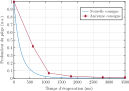
\includegraphics[width=0.7\textwidth]{Fig/Modif_exp/comparaison_consignes_evap.pdf}
\caption{\textbf{Comparaison de la nouvelle et de l'ancienne consigne d'évaporation du faisceau pince.} L'ancienne consigne, composée de cinq morceaux de rampe linéaire, est représentée en bordeaux. La nouvelle consigne, donnée par l'équation \ref{eq:nouvelle_consigne_evap} est représentée en bleu, possède une décroissance plus rapide que dans le cas de l'ancienne consigne. Elle permet de plus d'obtenir un condensat de Bose-Einstein plus rapidement.}
\label{fig:comparaison_consigne_evap}
\end{figure}

Par construction, la formule \ref{eq:nouvelle_consigne_evap} permet de mieux tirer parti du processus d'évaporation naturelle. Il est alors possible d'effectuer une évaporation plus rapide, réduisant l'impact de la durée de vie finie des atomes par collisions avec le gaz résiduel. 

Dans la suite, nous nous concentrerons sur les premières \SI{700}{\milli\second} de l'évaporation, qui correspondent à la durée nécessaire pour atteindre le seuil $\mathcal{D}\approx 1$, pour lequel une partie condensée apparaît. Au delà de ce seuil, l'approche classique pour laquelle les lois d'échelle ont été déterminées précédemment n'est plus valide.%\footnote{Dans le cadre d'une évaporation à $\eta$ constant, le taux de pertes à trois corps ne dépend pas de la vitesse à laquelle l'évaporation est effectuée.}.
 



\paragraph*{Évolution de la température}

L'évolution de la température du nuage\footnote{La détermination expérimentale de la température en présence du champ de lévitation, basée sur le principe de focalisation atomique, est détaillée dans l'annexe \ref{ch:anex_mesure_temp}.} au cours de l'évaporation est représentée figure \ref{fig:eta_constant}, et témoigne d'un refroidissement important au cours de l'évaporation, comme attendu. Nous avons superposé à ces mesures la profondeur estimée\footnote{Cette estimation provient de la calibration du piège optique présentée section \ref{sc:calibration_piege_optique}.} de la pince divisée par 10, sans paramètre ajustable. L'accord entre ces courbes est remarquable, validant ainsi l'approche d'une évaporation à $\eta=10$ constant. Ceci constitue une preuve du caractère adiabatique de notre évaporation, le nuage étant constamment dans un état de quasi-équilibre thermodynamique.

\begin{figure}
\centering
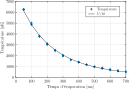
\includegraphics[width=0.7\textwidth]{Fig/Modif_exp/Evolution_température_eta.pdf}
\caption{\textbf{Évolution de la température au cours de l'évaporation.} La température (points bleus) est mesurée après différentes durées d'évaporation et comparée à la profondeur de piégeage du faisceau pince divisée par 10 (courbe noire). Sans paramètre ajustable, les deux courbes se superposent remarquablement.}
\label{fig:eta_constant}
\end{figure}







\paragraph*{Évolution du nombre d'atomes}

L'évolution du nombre d'atomes au cours de l'évaporation présente un intérêt particulier car celle-ci contient les informations liées aux processus de pertes inélastiques. Notamment, nous pouvons estimer le taux de pertes à trois corps à l'aide d'une mesure de la densité atomique et de la formule \ref{eq:pertes_atomes_3corps}. En comparant ces pertes aux variations mesurées du nombre d'atomes, on détermine que le rapport $R=\dot{N}_{\mathrm{3b}}/\dot{N}$ de l'ordre de 0.1, approximativement constant tout au long de l'évaporation. Il apparaît donc que les pertes à trois corps ont un effet marqué sur l'évolution du nombre d'atomes au cours de l'évaporation, mais que celles-ci ne constituent pas une limite pour notre système. 

De plus, il est possible de négliger l'effet des pertes dues aux collisions avec le gaz résiduel, limitant le temps de vie des atomes dans le piège à $1/\Gamma_{\mathrm{bg}}\approx\SI{10}{\second}$. En effet, l'optimisation de notre évaporation se concentre sur les premières \SI{700}{\milli\second} d'abaissement de la profondeur du piège\footnote{Cette durée correspond au temps nécessaire pour franchir le seuil de condensation $\mathcal{D}\approx 1$ et l'obtention d'un gaz dégénéré. Celle-ci était d'environ \SI{1.2}{\second} avec l'ancienne consigne.} comme illustré sur les figures \ref{fig:eta_constant} et \ref{fig:nombre_atomes_evap}, et la durée totale de notre évaporation est de \SI{3.5}{\second}, courte comparée au temps de vie permis par le gaz résiduel.

L'évolution du nombre d'atomes au cours de l'évaporation est représentée figure \ref{fig:nombre_atomes_evap} et est comparée à la prédiction de la loi d'échelle \ref{eq:scaling_atomes_3corps}, tracée avec les paramètres $\eta=10$ (déterminé précédemment grâce à l'évolution de la température au cours de l'évaporation) et $R=0.1$ (déterminé en estimant le taux de pertes à trois corps et rapporté aux pertes totales mesurées expérimentalement). Il apparaît donc que la théorie d'échelle permet de décrire correctement l'évolution du nombre d'atomes. 


\begin{figure}
\centering
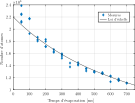
\includegraphics[width=0.7\textwidth]{Fig/modif_exp/Nombre_atomes_evap.pdf}
\caption{\textbf{Évolution du nombre d'atomes au cours de l'évaporation.} Les points bleus correspondent aux mesures expérimentales du nombre d'atomes, chaque point étant issu d'un unique cycle expérimental. La ligne continue noire correspond à la prédiction de la loi d'échelle \ref{eq:scaling_atomes_3corps} sans paramètre ajustable, avec les grandeurs $\eta=10$ et $R=0.1$ déterminées indépendamment. Il apparaît alors un très bon accord entre les données et le modèle.}
\label{fig:nombre_atomes_evap}
\end{figure}




\paragraph*{Évolution de la densité dans l'espace des phases}
Enfin, rappelons que l'optimisation de l'évaporation est réalisée en maximisant le gain de densité dans l'espace des phases par atome perdu, encodé par le paramètre $\gamma$. 

L'évolution de la densité dans l'espace des phases en fonction du nombre d'atomes est représentée figure \ref{fig:efficacite_evaporation_optique} en échelle logarithmique pour dans le cas de notre nouvelle consigne (en bleu) ainsi que pour notre ancienne consigne (en bordeaux). La comparaison est immédiate: la nouvelle consigne permet d'atteindre le seuil de condensation $\mathcal{D}\approx 1$ pour une perte d'atomes bien moindre que l'ancienne.

Plus quantitativement, l'efficacité mesurée pour la nouvelle consigne est de $\gamma\approx 4.5$ tandis que l'ancienne présente une efficacité d'environ 2.3\footnote{Cette mesure a été réalisée après le changement du laser source du piège optique. Avant changement, l'efficacité était plutôt estimée à 2.8 \citep{jendrzejewski2012quantum}.}, témoignant de la nette amélioration de notre évaporation. Notons que la loi d'échelle \ref{eq:efficacite_evap_3corps} en présence de pertes à trois corps prédit une valeur $\gamma\approx 6.5$, bien supérieure à notre valeur mesurée. Une étude approfondie de l'origine de cette différence n'a pas été menée compte-tenu de l'obtention récente de ces résultats et de l'excellente efficacité obtenue. En effet, la valeur de $\gamma\approx 3$ représente déjà une très bonne efficacité pour la plupart des expériences d'atomes ultra-froids \citep{barrett2001all}\citep{hung2008accelerating}.

Finalement, la consigne retenue à l'issue de l'optimisation de l'évaporation permet d'obtenir un condensat de Bose-Einstein d'environ \SI{1.2e6}{} atomes avec une température d'environ \SI{500}{\nano\kelvin} en \SI{700}{\milli\second}. Après \SI{3.5}{\second} d'évaporation, notre nuage contient environ \SI{2e5}{} atomes à une température de \SI{10}{\nano\kelvin} sans utiliser la technique d'ouverture adiabatique pour refroidir davantage. À l'heure de l'écriture de ces lignes, l'implémentation de cette technique avec la nouvelle consigne n'a pas encore été réalisée.


\begin{figure}
\centering
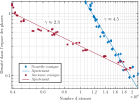
\includegraphics[width=0.8\textwidth]{Fig/Modif_exp/efficacité_évaporation_optique.pdf}
\caption{\textbf{Efficacité de l'évaporation optique.} En traçant la densité dans l'espace des phases du nuage en fonction du nombre d'atomes, on peut évaluer l'efficacité du refroidissement évaporatif. La nouvelle consigne d'évaporation permet d'obtenir les points bleus pour différents temps d'évaporation (jusqu'à \SI{700}{\milli\second}), tandis que l'ancienne consigne est représentée en bordeaux\protect\footnotemark\ (jusqu'à \SI{1.2}{\second}). Les lignes continues sont des ajustements des données expérimentales par des lois de puissance \ref{eq:efficacite_evaporation}, qui permettent ainsi d'extraire le paramètre $\gamma$ quantifiant l'efficacité de l'évaporation.}
\label{fig:efficacite_evaporation_optique}
\end{figure}
\footnotetext{Les données relatives à l'ancienne consigne ont été prises dans exactement les mêmes conditions expérimentales que celles relatives à la nouvelle: seule la consigne d'évaporation a été changée et ces données ont été obtenues les unes à la suite des autres.}

